\section{Test Case:User-defined Atmosphere Upwelling}
%====================================================

The user-defined atmosphere test case is sightly different for that of the built-in atmosphere in that the \texttt{TAPE5} uses defined surface emissivities and reflectivities, includes CFC profile information, and invokes the FFT scanning function.

\subsection{Double precision linux results}
%------------------------------------------
The double precision results for the linux/gfortran system for the user-defined atmosphere test case are shown in figure \ref{fig:run_example_user_defined_upwelling-dbl_gfortran}. Results using the AER \texttt{TAPE3} file were identical to the LNFL results. The linux/PGI runs produced identical results in all cases.

\begin{figure}[htp]
  \centering
  \qquad\sffamily\textbf{Verification Example: User-defined Atmosphere Upwelling}\\
  \qquad\sffamily\textbf{Red Hat linux platform; gfortran; double precision}\\
  \qquad\textsf{LBLRTM v11.3 brightness temperature difference for \textbf{Local} \texttt{TAPE3} run}\\
  \includegraphics[bb=82 490 534 648,clip,scale=1.0]{graphics/run_example_user_defined_upwelling/gfortran/dbl.eps}
  \qquad\textsf{LBLRTM v11.3 brightness temperature difference for \textbf{LNFL} \texttt{TAPE3} run}\\
  \includegraphics[bb=82 313 534 472,clip,scale=1.0]{graphics/run_example_user_defined_upwelling/gfortran/dbl.eps}
  \caption{User-defined Atmosphere Test: Comparison of the AER-supplied \texttt{TAPE27\_ex} output to the locally generated \texttt{TAPE27} output for the \textsl{double precision} version of LBLRTM v11.3 running on a Red Hat linux system using the gfortran compiler. \mbox{\textbf{(a)} Using} the little-endian \texttt{TAPE3} spectroscopic datafile generated from the local input shown in figure \ref{fig:local_tape3_tape5}. \mbox{\textbf{(b)} Using} the little-endian \texttt{TAPE3} spectroscopic datafile generated from the LNFL v2.5 distribution input shown in figure \ref{fig:lnfl_ex_tape3_tape5}. This result is identical to the same using the \textbf{AER} little-endian \texttt{TAPE3} spectroscopic datafile.}
  \label{fig:run_example_user_defined_upwelling-dbl_gfortran}
\end{figure}

The spectral location of the main feature in the brightness temperature differences using the locally generated \texttt{TAPE3}, figure \ref{fig:run_example_user_defined_upwelling-dbl_gfortran}(a), is at approximately 800\invcm{}. As with the built-in atmosphere test case, this residual is attributed to the different number of molecules in the two \texttt{TAPE3} files since the LNFL \texttt{TAPE3} run result in figure \ref{fig:run_example_user_defined_upwelling-dbl_gfortran}(b) does not contain the feature at 800\invcm.

A magnification of the LNFL \texttt{TAPE3} run result of figure \ref{fig:run_example_user_defined_upwelling-dbl_gfortran}(b) is shown in figure \ref{fig:run_example_user_defined_upwelling-dbl_gfortran_noyshare}. As is evident, the remaining residuals negligible.

\begin{figure}[htp]
  \centering
  \qquad\sffamily\textbf{Verification Example: User-defined Atmosphere Upwelling}\\
  \qquad\sffamily\textbf{Red Hat linux platform; gfortran; double precision}\\
  \qquad\textsf{LBLRTM v11.3 brightness temperature difference for \textbf{LNFL} \texttt{TAPE3} run}\\
  \includegraphics[bb=82 313 534 472,clip,scale=1.0]{graphics/run_example_user_defined_upwelling/gfortran/dbl_noyshare.eps}
  \caption{User-defined Atmosphere Test: A magnification of figure \ref{fig:run_example_user_defined_upwelling-dbl_gfortran}(b) showing the negligible residuals. This result is identical to the same using the \textbf{AER} big-endian \texttt{TAPE3} spectroscopic datafile. The PGI compiler also produced the same result.}
  \label{fig:run_example_user_defined_upwelling-dbl_gfortran_noyshare}
\end{figure}


\subsection{Double precision AIX results}
%-------------------------------------------

The double precision results for the IBM AIX system for the user-defined atmosphere test case are shown in figure \ref{fig:run_example_user_defined_upwelling-dbl_ibm}. Similar magnification of figure \ref{fig:run_example_user_defined_upwelling-dbl_ibm}(b) as seen in figure \ref{fig:run_example_user_defined_upwelling-dbl_gfortran_noyshare} show the IBM system produces the same residuals as the linux system.

\begin{figure}[htp]
  \centering
  \qquad\sffamily\textbf{Verification Example: User-defined Atmosphere Upwelling}\\
  \qquad\sffamily\textbf{IBM AIX platform; double precision}\\
  \qquad\textsf{LBLRTM v11.3 brightness temperature difference for \textbf{Local} \texttt{TAPE3} run}\\
  \includegraphics[bb=82 490 534 648,clip,scale=1.0]{graphics/run_example_user_defined_upwelling/ibm/dbl.eps}
  \qquad\textsf{LBLRTM v11.3 brightness temperature difference for \textbf{LNFL} \texttt{TAPE3} run}\\
  \includegraphics[bb=82 313 534 472,clip,scale=1.0]{graphics/run_example_user_defined_upwelling/ibm/dbl.eps}
  \caption{User-defined Atmosphere Test: Comparison of the AER-supplied \texttt{TAPE27\_ex} output to the locally generated \texttt{TAPE27} output for the \textsl{double precision} version of LBLRTM v11.3 running on an IBM AIX system. \mbox{\textbf{(a)} Using} the big-endian \texttt{TAPE3} spectroscopic datafile generated from the local input shown in figure \ref{fig:local_tape3_tape5}. \mbox{\textbf{(b)} Using} the big-endian \texttt{TAPE3} spectroscopic datafile generated from the LNFL v2.5 distribution input shown in figure \ref{fig:lnfl_ex_tape3_tape5}. This result is identical to the same using the \textbf{AER} big-endian \texttt{TAPE3} spectroscopic datafile.}
  \label{fig:run_example_user_defined_upwelling-dbl_ibm}
\end{figure}


\subsection{Single precision run results}
%----------------------------------------

The single precision results for both the linux and AIX systems for the user-supplied atmosphere test case are shown in figures \ref{fig:run_example_user_defined_upwelling-sgl_gfortran} and \ref{fig:run_example_user_defined_upwelling-sgl_ibm} respectively.

\begin{figure}[htp]
  \centering
  \qquad\sffamily\textbf{Verification Example: User-defined Atmosphere Upwelling}\\
  \qquad\sffamily\textbf{Red Hat linux platform; gfortran; single precision}\\
  \qquad\textsf{LBLRTM v11.3 brightness temperature difference for \textbf{Local} \texttt{TAPE3} run}\\
  \includegraphics[bb=82 490 534 648,clip,scale=1.0]{graphics/run_example_user_defined_upwelling/gfortran/sgl.eps}
  \qquad\textsf{LBLRTM v11.3 brightness temperature difference for \textbf{LNFL} \texttt{TAPE3} run}\\
  \includegraphics[bb=82 313 534 472,clip,scale=1.0]{graphics/run_example_user_defined_upwelling/gfortran/sgl.eps}
  \caption{User-defined Atmosphere Test: Comparison of the AER-supplied \texttt{TAPE27\_ex} output to the locally generated \texttt{TAPE27} output for the \textsl{single precision} version of LBLRTM v11.3 running on a Red Hat linux system using the gfortran compiler. \mbox{\textbf{(a)} Using} the little-endian \texttt{TAPE3} spectroscopic datafile generated from the local input shown in figure \ref{fig:local_tape3_tape5}. \mbox{\textbf{(b)} Using} the little-endian \texttt{TAPE3} spectroscopic datafile generated from the LNFL v2.5 distribution input shown in figure \ref{fig:lnfl_ex_tape3_tape5}. This result is identical to the same using the \textbf{AER} little-endian \texttt{TAPE3} spectroscopic datafile.}
  \label{fig:run_example_user_defined_upwelling-sgl_gfortran}
\end{figure}

\begin{figure}[htp]
  \centering
  \qquad\sffamily\textbf{Verification Example: User-defined Atmosphere Upwelling}\\
  \qquad\sffamily\textbf{IBM AIX platform; single precision}\\
  \qquad\textsf{LBLRTM v11.3 brightness temperature difference for \textbf{Local} \texttt{TAPE3} run}\\
  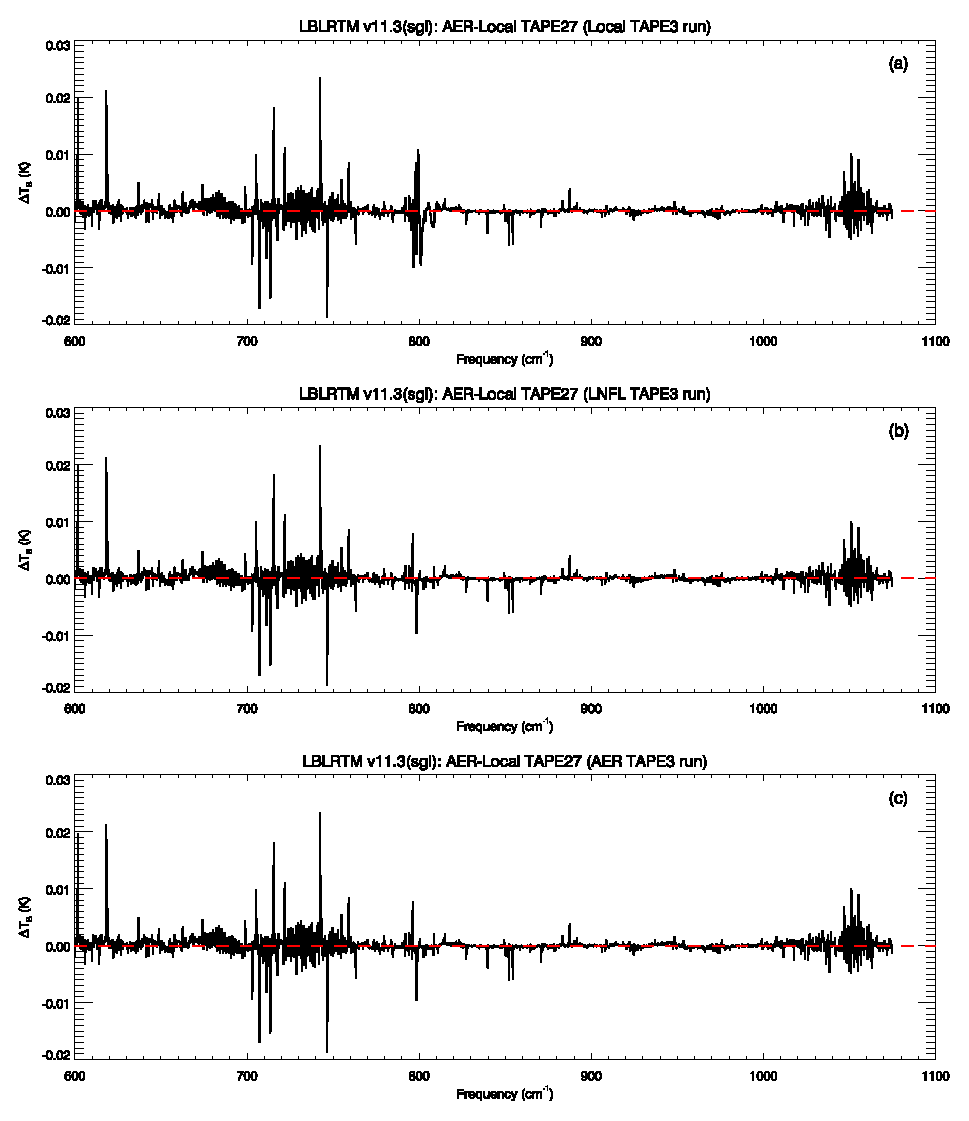
\includegraphics[bb=82 490 534 648,clip,scale=1.0]{graphics/run_example_user_defined_upwelling/ibm/sgl.eps}
  \qquad\textsf{LBLRTM v11.3 brightness temperature difference for \textbf{LNFL} \texttt{TAPE3} run}\\
  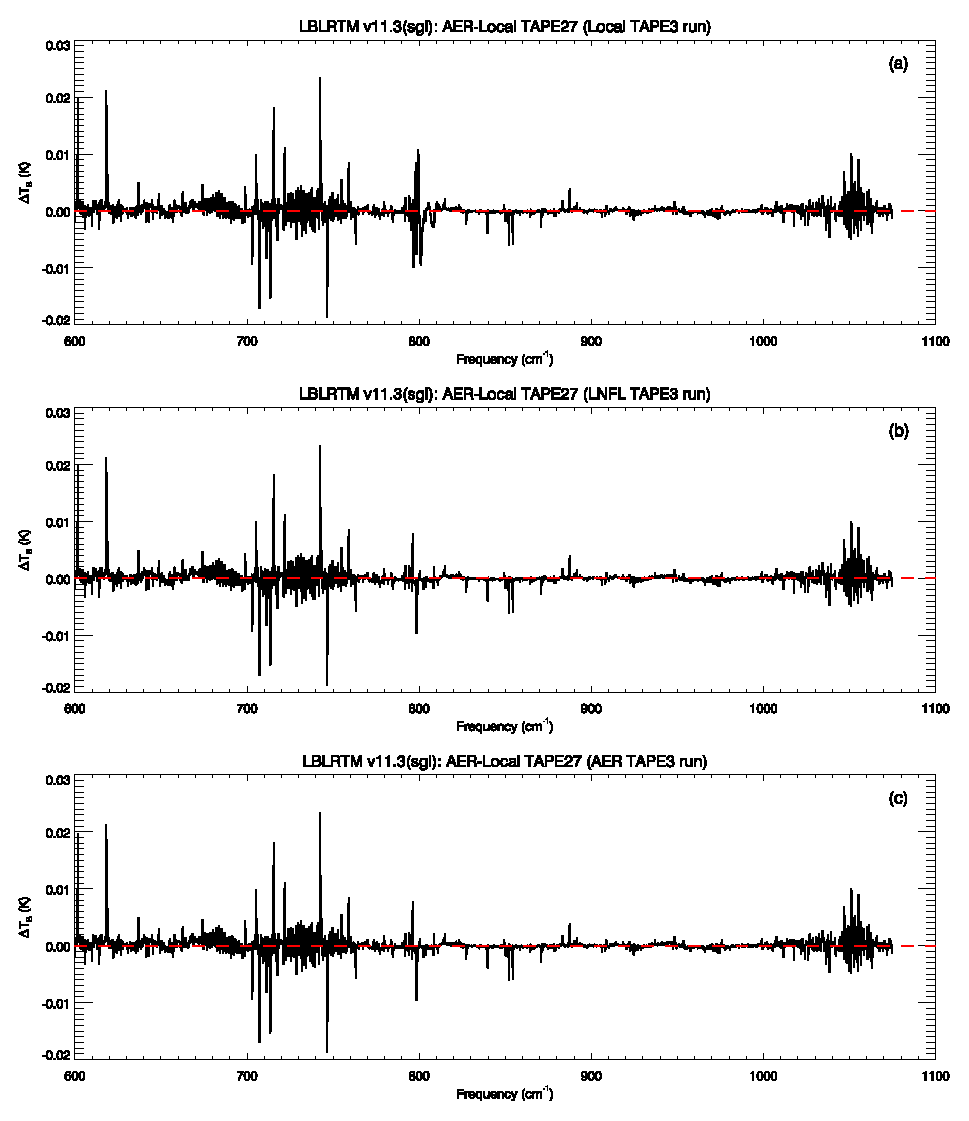
\includegraphics[bb=82 313 534 472,clip,scale=1.0]{graphics/run_example_user_defined_upwelling/ibm/sgl.eps}
  \caption{User-defined Atmosphere Test: Comparison of the AER-supplied \texttt{TAPE27\_ex} output to the locally generated \texttt{TAPE27} output for the \textsl{single precision} version of LBLRTM v11.3 running on an IBM AIX system. \mbox{\textbf{(a)} Using} the big-endian \texttt{TAPE3} spectroscopic datafile generated from the local input shown in figure \ref{fig:local_tape3_tape5}. \mbox{\textbf{(b)} Using} the big-endian \texttt{TAPE3} spectroscopic datafile generated from the LNFL v2.5 distribution input shown in figure \ref{fig:lnfl_ex_tape3_tape5}. This result is identical to the same using the \textbf{AER} big-endian \texttt{TAPE3} spectroscopic datafile.}
  \label{fig:run_example_user_defined_upwelling-sgl_ibm}
\end{figure}


The feature due to using the locally generated \texttt{TAPE3} file is present at around 800\invcm{} in both the linux and AIX runs. However, other than that, the two platforms yield very similar results. The character of the single precision residuals for this case are also different. Recall that the built-in atmosphere test case residuals for the single precision test case (see section \ref{sec:built_in_sgl}) indicated there was a frequency shift in the output \texttt{TAPE27} data files. That is not the case here. A magnification of figure \ref{fig:run_example_user_defined_upwelling-sgl_gfortran}(b) is shown in figure \ref{fig:run_example_user_defined_upwelling-sgl_700-770} for 700-770\invcm, and in figure \ref{fig:run_example_user_defined_upwelling-sgl_900-1000} for 900-1000\invcm. There does appear to be some residual low spectral resolution feature in figure \ref{fig:run_example_user_defined_upwelling-sgl_900-1000}. It is not known what is causing this feature (CFC absorption differences?) but the magnitude is of the order of millikelvin so no further investigation will be undertaken.

\begin{figure}[htp]
  \centering
  \qquad\sffamily\textbf{Verification Example: User-define Atmosphere Upwelling}\\
  \qquad\sffamily\textbf{Red Hat linux platform; gfortran; single precision}\\
  \qquad\textsf{LBLRTM v11.3 brightness temperature difference for \textbf{LNFL} \texttt{TAPE3} run}\\
  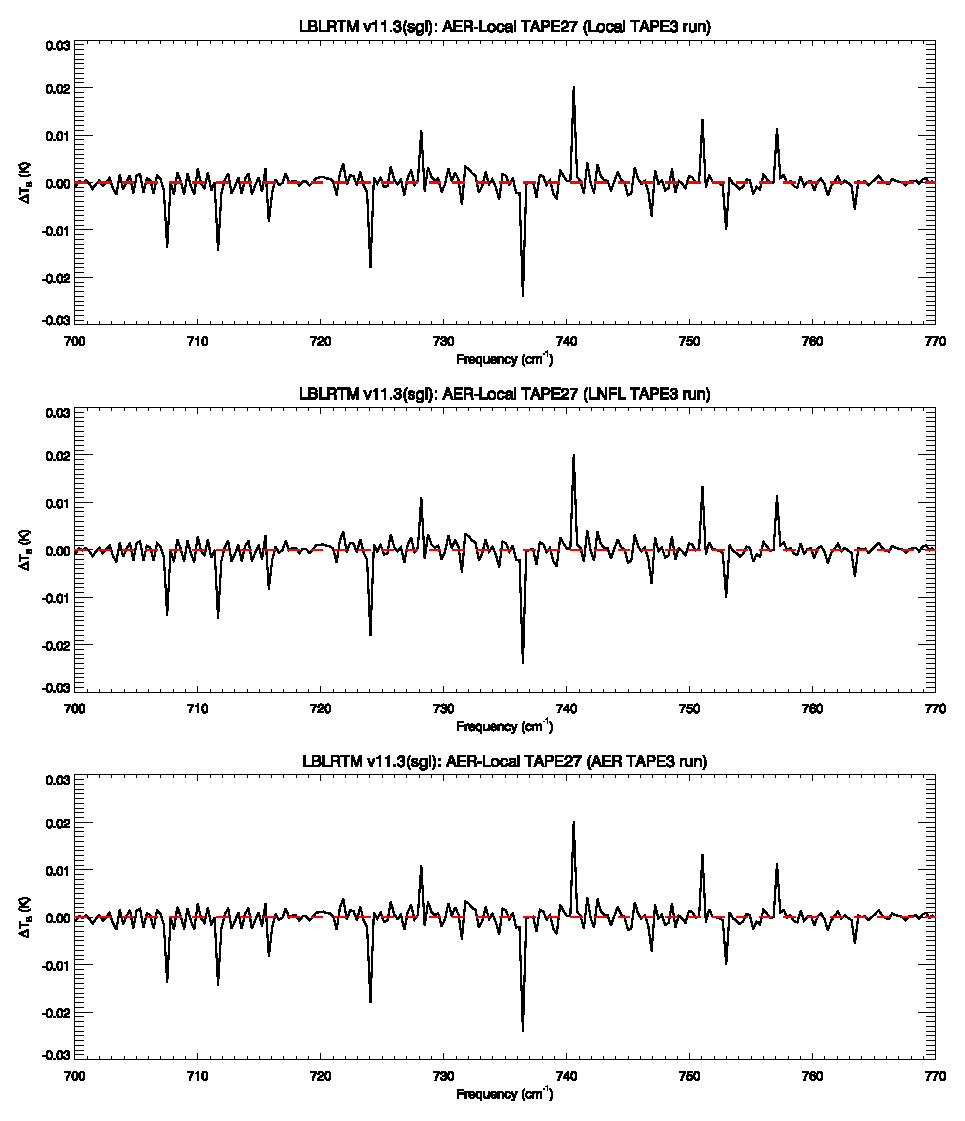
\includegraphics[bb=82 313 534 472,clip,scale=1.0]{graphics/run_example_user_defined_upwelling/gfortran/sgl_700-770.eps}
  \caption{User-defined Atmosphere Test: A magnification of the 700-770\invcm{} spectral region from figure \ref{fig:run_example_user_defined_upwelling-sgl_gfortran}(b). The character of the differences does not indicate a frequency shift (as seen in figure \ref{fig:run_example_built_in_atm_upwelling-sgl_gfortran_1125-1127}).}
  \label{fig:run_example_user_defined_upwelling-sgl_700-770}
\end{figure}

\begin{figure}[htp]
  \centering
  \qquad\sffamily\textbf{Verification Example: User-define Atmosphere Upwelling}\\
  \qquad\sffamily\textbf{Red Hat linux platform; gfortran; single precision}\\
  \qquad\textsf{LBLRTM v11.3 brightness temperature difference for \textbf{LNFL} \texttt{TAPE3} run}\\
  \includegraphics[bb=82 313 534 472,clip,scale=1.0]{graphics/run_example_user_defined_upwelling/gfortran/sgl_900-1000.eps}
  \caption{User-defined Atmosphere Test: A magnification of the 900-1000\invcm{} spectral region from figure \ref{fig:run_example_user_defined_upwelling-sgl_gfortran}(b). The cause of the low spectral resolution feature is not known (CFC absorption differences?).}
  \label{fig:run_example_user_defined_upwelling-sgl_900-1000}
\end{figure}
